\documentclass[UTF8]{report}
\usepackage{amsmath}
\usepackage{cite}
\usepackage{algorithm}
\usepackage{algorithmicx}
\usepackage{algpseudocode}
\usepackage{lipsum,float}
\usepackage{geometry}
\usepackage{graphicx} %use graph format
\usepackage{epstopdf}
\usepackage{float}
\usepackage{subfigure}
\usepackage{listings}
\usepackage{color}
\definecolor{dkgreen}{rgb}{0,0.6,0}
\definecolor{gray}{rgb}{0.5,0.5,0.5}
\definecolor{mauve}{rgb}{0.58,0,0.82}
\lstset{breaklines}%自动将长的代码行换行排版
\lstset{ %
extendedchars=false,            % Shutdown no-ASCII compatible
language=Matlab,                % choose the language of the code
basicstyle=\footnotesize\tt,    % the size of the fonts that are used for the code
tabsize=3,                            % sets default tabsize to 3 spaces
numbers=left,                   % where to put the line-numbers
numberstyle=\tiny,              % the size of the fonts that are used for the line-numbers
stepnumber=1,                   % the step between two line-numbers. If it's 1 each line
                                % will be numbered
numbersep=5pt,                  % how far the line-numbers are from the code   %
keywordstyle=\color[rgb]{0,0,1},                % keywords
commentstyle=\color[rgb]{0.133,0.545,0.133},    % comments
stringstyle=\color[rgb]{0.627,0.126,0.941},      % strings
backgroundcolor=\color{white}, % choose the background color. You must add \usepackage{color}
showspaces=false,               % show spaces adding particular underscores
showstringspaces=false,         % underline spaces within strings
showtabs=false,                 % show tabs within strings adding particular underscores
frame=single,                 % adds a frame around the code
captionpos=b,                   % sets the caption-position to bottom
breaklines=true,                % sets automatic line breaking
breakatwhitespace=false,        % sets if automatic breaks should only happen at whitespace
title=\lstname,                 % show the filename of files included with \lstinputlisting;
                                % also try caption instead of title
mathescape=true,escapechar=?    % escape to latex with ?..?
escapeinside={\%*}{*)},         % if you want to add a comment within your code
%columns=fixed,                  % nice spacing
%morestring=[m]',                % strings
%morekeywords={%,...},%          % if you want to add more keywords to the set
%    break,case,catch,continue,elseif,else,end,for,function,global,%
%    if,otherwise,persistent,return,switch,try,while,...},%
}
\geometry{a4paper,left=2.5cm,right=2.5cm,top=2.5cm,bottom=2.5cm}
\renewcommand{\bibname}{Reference}

\title{\Huge \textbf{QR Algorithm}}
\author{Jingxiang Wu}
\date{\today}
\makeatletter
\newenvironment{breakablealgorithm}
  {% \begin{breakablealgorithm}
   \begin{center}
     \refstepcounter{algorithm}% New algorithm
     \hrule height.8pt depth0pt \kern2pt% \@fs@pre for \@fs@ruled
     \renewcommand{\caption}[2][\relax]{% Make a new \caption
       {\raggedright\textbf{\ALG@name~\thealgorithm} ##2\par}%
       \ifx\relax##1\relax % #1 is \relax
         \addcontentsline{loa}{algorithm}{\protect\numberline{\thealgorithm}##2}%
       \else % #1 is not \relax
         \addcontentsline{loa}{algorithm}{\protect\numberline{\thealgorithm}##1}%
       \fi
       \kern2pt\hrule\kern2pt
     }
  }{% \end{breakablealgorithm}
     \kern2pt\hrule\relax% \@fs@post for \@fs@ruled
   \end{center}
  }
\makeatother
\begin{document}\large
\maketitle
\tableofcontents
\chapter{Traditional QR Algorithm with double and more shifts}

In this chapter,we will talk about the traditional QR Algorithm with double and more shifts, giving complete algorithm and related details of this algorithm.
\section{The Double-Implict-Shift Strategy}
\textbf{The Double-Implict-Shift Strategy}\cite{QR1,QR2}is published by Francis in 1961-1962, which proposed how to compute a real schur-decomposition.
First, we take a hessenberg decomposition to a dense matrix for making it an almost upper quasi-triangular matrix, see \textbf{Algorithm 1}
\input{Hessenberg}

And then selected shifts as the eigenvalues of a trailing principal 2\(\times\)2 submatrix, the detailed algorithm see \textbf{Algorithm 2}
\renewcommand{\algorithmicrequire}{\textbf{Input:}}
\renewcommand{\algorithmicensure}{\textbf{Output:}}
\begin{breakablealgorithm}
  \caption{Double-shift-QR-iteration}
  \label{alg::Double-shift-QR-iteration}
  \begin{algorithmic}[1]
    \Require $H$: a hessenberg matrix
    \Ensure $H$: a hessenberg matrix;$W$: a n*3 matrix, stored n-1 household vectors
    \State\(s=H(n-1,n-1)+H(n,n)\)
    \State\(t=H(n-1,n-1)H(n,n)-H(n,n-1)H(n,n-1)\)
    \State\(x=H(1,1)H(1,1)+H(1,2)H(2,1)-sH(1,1)+t\)
    \State\(y=H(2,1)(H(1,1)+H(2,2)-s)\)
    \State\(z=H(2,1)H(3,2)\)
    \State\(vector=[x;y;z]\)
    \For{$k=0$ to $n-3$}
      \State\(w=house(vector)\)
      \State\(q=max[1,k]\)
      \State\(r=min[k+4,n]\)
      \State\(W(1:3,k+1)=w\);   
      \State\(H(k+1:k+3,q:n)=(I-2w{w^T})H(k+1:k+3,q:n)\)
      \State\(H(1:r,k+1:k+3)=H(1:r,k+1:k+3)(I-2w{w^T})\)
      \State\(x=H(k+2,k+1)\);
      \State\(y=H(k+3,k+1)\);
      \If {\(k<n-3\)} 
      \State \(vector=[x;y;z]\)
      \EndIf
    \EndFor
      \State\(w=household([x;y])\);
      \State\(W(1:2,n-1)=w\)
      \State\(H(n-1:n,n-2:n)=(I-2w{w^T})H(n-1:n,n-2:n)\)
      \State\(H(1:n,n-1:n)=H(1:n,n-1:n)(I-2w{w^T})\)
  \end{algorithmic}
\end{breakablealgorithm}

After some steps iteration, we can find convergence in both upper left and lower right of this matrix, and after each iteration, it converge at most two eigenvalues in the upper left corner and lower right corner of the matrix.

When it converge only one eigenvalue, it must be a real eigenvalue; when it converge two eigenvalue, most cases we get a pair of conjugate complex eigenvalues. But in some cases, the \(H(m,m-1)\) is not small enough while the \(H(m-1,m-2)\) is small enough, such as:
\[\left( {\begin{array}{*{20}{c}}
 \times & \times & \times \\
{{{10}^{ - 15}}}& \times & \times \\
0&{{{10}^{ - 7}}}& \times 
\end{array}} \right)\]

In this case, we can compute a \({2 \times 2}\) matrix \({\widetilde Q}\) in \({O(1)}\) time and put it onto $Q$,\(H(1:i-1,i:m)\) and \(H(i:m,m+1:n)\), such that:
\[\left( {\begin{array}{*{20}{c}}
 \times & \times \\
{{{10}^{ - 7}}}& \times 
\end{array}} \right)\widetilde Q = \widetilde Q\left( {\begin{array}{*{20}{c}}
{{\lambda _1}}& \times \\
0&{{\lambda _2}}
\end{array}} \right)\]

For a \({2 \times 2}\) matrix which have a pair of conjugate complex eigenvalues \(a + bi\), in this case, we can compute a \({2 \times 2}\) matrix \({\widetilde Q}\) in \({O(1)}\) time and put it onto $Q$,\(H(1:i-1,i:m)\) and \(H(i:m,m+1:n)\), such that:
\[\left( {\begin{array}{*{20}{c}}
 \times & \times \\
 \times & \times 
\end{array}} \right)\widetilde Q = \widetilde Q\left( {\begin{array}{*{20}{c}}
a&m\\
t&a
\end{array}} \right)\]

And at last, if \(m>i\) still be true, compute the real schur decompetition of last \({2 \times 2}\) matrix. In these three cases, the orthogonal matrix can be analytically obtained. Based on the above process, we can conclude the following \textbf{Algorithm 3}
\renewcommand{\algorithmicrequire}{\textbf{Input:}}
\renewcommand{\algorithmicensure}{\textbf{Output:}}
\begin{breakablealgorithm}
  \caption{Double-shift-QR-algorithm}
  \label{alg::Double-shift-QR-algorithm}
  \begin{algorithmic}[1]
  \Require $A$:a dense matrix; $flag$:flag equals 0 means this matrix is a hessenberg matrix
  \Ensure $E$:all eigenvalue of A;$H$:a real-schur form matrix;$Q$:orthogonal transform matrix satisfy \(AQ=QH\)
  \State\(Q={I_n}\);
  \If {\(flag=1\)}
    \State\([Q,H]=hessenberg(H)\)
  \EndIf
  \State\(i=1\);
  \State\(m=n\);
  \State\(tol={10^{-15}}\);
  \While{\(m-i+1>2\)}
  \State\([W,H(i:m,i:m)]=\)double-shift-QR-iteration(\(H(i:m,i:m)\));
  \State put these household vector to orthogonal transform matrix $Q$,\(H(1:i-1,i:m)\) and \(H(i:m,m+1:n)\)
  \State Finding converged eigenvalues in the upper left corner of (\(H(i:m,i:m)\))
  \State Finding converged eigenvalues in the lower right corner of (\(H(i:m,i:m)\))
  \If{There is no converged eigenvalue}
    \State Continue
  \EndIf
  \If{a real eigenvalue converges}
    \If{\(H(i+1,i)<tol\)}
      \State\(E(i,1)=H(i,i)\)
      \State\(i=i+1\)
    \EndIf
   \If{\(H(m,m-1)<tol\)}
      \State\(E(m,1)=H(m,m)\)
      \State\(m=m-1\)
    \EndIf
  \EndIf
  \If{two eigenvalues converge}
    \If{\(H(i+2,i+1)<tol\)}
      \State Judge whether this 2\(\times\)2 matrix has two real eigenvalues or a pair of conjugate complex eigenvalues
      \State Compute eigenvalue of this 2\(\times\)2 matrix
      \State\(i=i+2\)
    \EndIf
   \If{\(H(m-1,m-2)<tol\)}
      \State Judge whether this 2\(\times\)2 matrix has two real eigenvalues or a pair of conjugate complex eigenvalues
      \State Compute eigenvalue of this 2\(\times\)2 matrix
      \State\(m=m-2\)
    \EndIf
  \EndIf
  \EndWhile
  \If{\(m>i)\)}
    \State Judge whether this least 2\(\times\)2 matrix has two real eigenvalues or a pair of conjugate complex eigenvalues
    \State Compute real-schur form of this least 2\(\times\)2 matrix
    \State Put \(U\in{R^{2\times 2}}\)to $Q$,\(H(1:i-1,i:m)\) and \(H(i:m,m+1:n)\)
  \EndIf
  \end{algorithmic}
\end{breakablealgorithm}
(In the Matlab source code, I use the build-in function \(schur\) to solve \({2 \times 2}\) matrix)
\section{The Sextuple-Implicit-Shift Strategy}
To get faster convergence speed and higher computational efficiency, we are unsatisfied with introducing two shifts each time. According to the same principle, people proposed Multishift QR Algorithm. In this section, we introduce and implement the Sextuple-Implicit-Shift Strategy.

As we all know, Implicit QR decomposition use a conclusion in Arnoldi process-the first column determines the whole orthogonal matrix \(Q\). So we construct a vector as a start, this vector is:
\[\prod\limits_{i = 1}^k {(H - {\lambda _i}I){e_1}} \]

Noticed that the matrix \(\prod\limits_{i = 1}^k {(H - {\lambda _i}I)} \) is the value of characteristic polynomial of \(k\times k\) trailing principal submatrix at \(H\), we can get characteristic polynomial of \(k\times k\) trailing principal submatrix with symbolic computation. Then we can prove that the vector only have k+1 non-zero elements, which is uniquely determined by \(H(1:k+1,1:k+1)\), so we can use build-in function \(poly\) and \(polyvalm\) in Matlab to compute this vector. Then do household transformation along with the diagonal line like Double-Implict-Shift. The detailed algorithm see \textbf{Algorithm 4}:
\renewcommand{\algorithmicrequire}{\textbf{Input:}}
\renewcommand{\algorithmicensure}{\textbf{Output:}}
\begin{breakablealgorithm}
  \caption{Sextuple-shift-QR-iteration}
  \label{alg::Sextuple-shift-QR-iteration}
  \begin{algorithmic}[1]
    \Require $H$: a hessenberg matrix
    \Ensure $H$: a hessenberg matrix;$W$: a n*6 matrix, stored n-1 household vectors
    \State\(a=poly(H(n-5:n,n-5:n))\)
    \State\(vector=polyvalm(a,H(1:7,1:7))\)
    \For{$k=0$ to $n-3$}
      \State\(w=household(vector)\)
      \State\(q=max[1,k]\)
      \State\(r=min[k+8,n]\)
      \State\(W(1:7,k+1)=w\);   
      \State\(H(k+1:k+7,q:n)=(I-2w{w^T})H(k+1:k+7,q:n)\)
      \State\(H(1:r,k+1:k+7)=H(1:r,k+1:k+7)(I-2w{w^T})\)
      \If {\(k<n-7\)} 
      \State \(vector=H(k+2:k+8,k+1)\)
      \EndIf
    \EndFor
    \For{$i=1$ to $5$}
      \State\(w=household(H(n-6+i:n,n-7+i))\);
      \State\(W(1:7-i,n-6+i)=w\)
      \State\(H(n-6+i:n,n-7+i:n)=(I-2w{w^T})H(n-6+i:n,n-7+i:n)\)
      \State\(H(1:n,n-6+i:n)=H(1:n,n-6+i:n)(I-2w{w^T})\)
    \EndFor
  \end{algorithmic}
\end{breakablealgorithm}

After some steps iteration, we can find convergence in both upper left and lower right of this matrix, but in Sextuple-shift-QR-iteration, it is possible to converge k eigenvalues in the upper left and lower right corner of this matrix, \(k\le6\). Then we solve schur decomposition for the matrices of order no more than six by Double-shift-QR-Algorithm. Based on the above process, we can conclude the following \textbf{Algorithm 5}:
\renewcommand{\algorithmicrequire}{\textbf{Input:}}
\renewcommand{\algorithmicensure}{\textbf{Output:}}
\begin{breakablealgorithm}
  \caption{Sextuple-shift-QR-algorithm}
  \label{alg::Sextuple-shift-QR-algorithm}
  \begin{algorithmic}[1]
  \Require $A$:a dense matrix; $flag$:flag equals 0 means this matrix is a hessenberg matrix
  \Ensure $E$:all eigenvalue of A;$H$:a real-schur form matrix;$Q$:orthogonal transform matrix satisfy \(AQ=QH\)
  \State\(Q={I_n}\);
  \If {\(flag=1\)}
    \State\([Q,H]=hessenberg(H)\)
  \EndIf
  \State\(i=1\);
  \State\(m=n\);
  \State\(tol={10^{-15}}\);
  \While{\(m-i+1>6\)}
  \State\([W,H(i:m,i:m)]=\)double-shift-QR-iteration(\(H(i:m,i:m)\));
  \State put these household vector to orthogonal transform matrix $Q$,\(H(1:i-1,i:m)\) and \(H(i:m,m+1:n)\)
  \State Finding eigenvalues of converged in the upper left corner of (\(H(i:m,i:m)\))
  \State Finding eigenvalues of converged in the lower right corner of (\(H(i:m,i:m)\))
  \If{There is no converged eigenvalue}
    \State Continue
  \EndIf
  \State Suppose the number of converged eigenvalues is k,\(k\le6\)
  \State use Double-shift-QR-algorithm to \(H(m-k+1:m,m-k+1:m)\), put \(\widetilde Q\) to \(H(1:m-k,m-k+1:m)\),\(H(m-k+1:m,m+1:n)\),\(Q(1:n,m-k+1:m)\)
  \EndWhile
  \If{\((m>i)\)}
    \State use Double-shift-QR-algorithm to\(H(i:m,i:m)\), put \(\widetilde Q\) to\(H(1:i-1,i:m)\),\(H(i:m,m+1:n)\),\(Q(1:n,i:m)\)
  \EndIf
  \end{algorithmic}
\end{breakablealgorithm}
The numerical experiments see \textbf{chapter 3}, and the Matlab source code see \textbf{The Appendix B}.
\chapter{Aggressive Early Defaltion for The Multishift QR Algorithm}
In this chapter, we will talk about The Multishift QR Algorithm based on BLAS 3 performance and Aggressive Early Deflation Strategy, which is a really aggressive but correct strategy. These methods help us to solve dense unsymmetric matrices of size several thousands without losing too much accuracy.
\section{The small-bulge multishift QR Algorithm}\cite{MQRC}
Find the largest non-negative q and the samllest non-negative p such that:
\[\begin{array}{*{20}{c}}
{H = \left[ {\begin{array}{*{20}{c}}
{{H_{11}}}&{{H_{12}}}&{{H_{13}}}\\
0&{{H_{22}}}&{{H_{23}}}\\
0&0&{{H_{33}}}
\end{array}} \right]}&{\begin{array}{*{20}{c}}
p\\
{n-p-q}\\
q
\end{array}}\\
{\begin{array}{*{20}{c}}
p&{n-p-q}&q
\end{array}}&{}
\end{array}\]
Where \(H_{33}\) is upper quasi-triangular and \(H_{22}\) is unreduced.

For using BLAS 3 performance in QR iteration, we tend to choose more shifts and longer shifts distance each time to update \(Q\), \(H_{12}\) and \(H_{23}\). Unfortunately, if we choose too more shifts every time, the computation will be inaccurate, while a large-bulge will cause m times rounding error to a small-bugle. So we choose small-bulge multishift QR Strategy.

First, we choose \(2m\) shifts and choose a pair of complex conjugate eigenvalues or two real eigenvalues every time, and put it to the appropriate position. This process will construct a medium-sized orthogonal transformation matrice, use it to update the right side of the long strip-like matrix, which can be computed by BLAS 3.

Then, we move the m small-bugles k steps each time, this process will construct a medium-sized orthogonal transformation matrice, use it to update both the right and the top side of the long strip-like matrix, which can be computed by BLAS 3.At the same time, it should be noted that the remaining space may not be enough to move k steps when we are close to the lower right corner.

At last, remove bugles in the order in which they are introduced, use the medium-sized orthogonal transformation matrice to update the top side of the long strip-like matrix. The detailed algorithm see \textbf{Algorithm 6}
\renewcommand{\algorithmicrequire}{\textbf{Input:}}
\renewcommand{\algorithmicensure}{\textbf{Output:}}
\begin{breakablealgorithm}
  \caption{Double-shift-chasing-iteration}
  \label{alg::Double-shift-chasing-iteration}
  \begin{algorithmic}[1]
    \Require $H$: a hessenberg matrix;
    \Ensure 
    $H$: a hessenberg matrix;

    $m$: we use 2m shifts;
    $k$: the length for each move;

    $Ava$:do Ava full movings;
    $least$:do a moving at last with length of least

    $W$: a three-dimensional array, stored orthogonal transform matrix
    \State choose m and k and compute Ava and least
    \State choose 2m eigenvalue
    \For{$i=1$ to $m$}
    \State use a pair of complex conjugate eigenvalues or two real eigenvalues to create a vector, transform it to the position \(3*m-i,3*m-i\)
    \State compute orthogonal transform matrix \({\widetilde Q}\) with order of \(3m+1\)
    \EndFor
    \State put \({\widetilde Q}\) to \(H(1:3m+1,3m+2:n)\)
    \For {$i=1$ to $Ava$}
    \For {$t=1$ to $k$}
    \State move \({{t^{th}}}\) small-bulge down along with the diagonal line k-steps at once
    \State compute orthogonal transform matrix \({\widetilde Q}\) with order of \(3m+k+1\)
    \EndFor
    \State put \({\widetilde Q}\) to \(H(1:k(i-1),1+k(i-1):3m+ki+1)\) and \(H(1+k(i-1):3m+ki+1,3m+ki+2:n)\)
    \EndFor
    \For {$t=1$ to $least$}
\State move \(t^{th}\) small-bulge down along with the diagonal line least-steps at once
    \State compute orthogonal transform matrix \({\widetilde Q}\) with order of \(3m+k+1\)
    \EndFor
    \State put \({\widetilde Q}\) to \(H(1:ki,1+ki:n)\)
    \For {$i=m$ to $1$}
    \State Starting at the bottom of the matrix, apply each small-bulge to the bottom of the matrix.
    \State compute orthogonal transform matrix \({\widetilde Q}\) with order of \(3m+1\)
    \EndFor
    \State put \({\widetilde Q}\) to \(H(1:n-3m-1,n-3m:n)\)
 \end{algorithmic}
\end{breakablealgorithm}

Suppose the order of the matrix is n, we can get The amount of calculation done with BLAS 3 is:
\[\begin{array}{l}
2{(3m + 1)^2}(n - 3m - 1) + \sum\limits_{i = 1}^{\frac{{n - 3m - 1}}{k}} {{{(3m + k + 1)}^2}(k(i - 1) + n - 3m - ki - 1)} \\
 = \frac{{n - 3m - 1}}{k}({(3m + k + 1)^2}(n - (3m + k + 1)) + 2k{(3m + 1)^2})
\end{array}\]

The amount of calculation done with BLAS 2 is:
\[{(3m + k + 1)^3}\frac{{n - 3m - 1}}{k} + 2{(3m + 1)^3}\]

Choose \(m = \left\lfloor {\sqrt n } \right\rfloor \)and \(k = 3m\). Then we can simplify the above equation:
\[\begin{array}{l}
BLAS - 2:216{n^2} - 162n\sqrt n \\
BLAS - 3:36{n^2}\sqrt n  - 270{n^2} + 486n\sqrt n 
\end{array}\]

This shows us that the computation in BLAS-3 is much more than BLAS-2 under this choice.
\section{Aggressive Early Deflation and the details for choices of shifts}\cite{AED}
The Aggressive Early Deflation, a strategy for trailing principal submatrix convergence, can increase the speed of convergence.

Suppose we use some eigenvalues of \(H_{33}\) to do a small-bulge multishift QR iteration, (the order of \(H_{33}\) should be bigger than the number of shifts), and H can be expressed as:
\[\begin{array}{*{20}{c}}
{H = \left[ {\begin{array}{*{20}{c}}
{{H_{11}}}&{{H_{12}}}&{{H_{13}}}\\
0&{{H_{22}}}&{{H_{23}}}\\
0&{{H_{23}}}&{{H_{33}}}
\end{array}} \right]}&{\begin{array}{*{20}{c}}
{n - p - 1}\\
1\\
p
\end{array}}\\
{\begin{array}{*{20}{c}}
{n - p - 1}&1&p
\end{array}}&{}
\end{array}\]
Where \(H_{23}\) is a vector with only one non-zero element at the first position.

Now we do an assumable strategy: Do a real-schur decomposition to \(H_{33}\), this action will recursively call the program that solves the real-schur decomposition, until this matrix is small enough to use the Sextuple-Shift-QR-Algorithm.

Just suppose we finish this programm, which means we can call this function to get real-schur decomposition of \(H_{33}\) and orthogonal transformation matrix \(\widetilde Q\), put this matrix to \(H_{32}\) and you can get a full vector. After observation, it was found that this vector has many elements close to 0, which usually concentrated at the bottom of the vector, of course, sometimes it appears in the middle of the vector. Meanwhile, there are still some elements of are not near to zero. The index of the element in the vector corresponds to the position of the eigenvalue in the upper quasi-triangular matrix, and the vector elements corresponding to a pair of eigenvalues of a conjugate complex eigenvalues will converges at the same time. Then if converged element is not at the bottom of vector, do a \(orderschur\) to swap it to the bottom.(This process is not programmed by me, because I observed that in most cases, eigenvalues converge from bottom to top.) If there are enough eigenvalues converge, we put this orthogonal transformation matrix \(\widetilde Q\) to \(\left[ {\begin{array}{*{20}{c}}
{{H_{13}}}\\
{{H_{23}}}
\end{array}} \right]\) and \(H_{32}\). Then the matrix becomes the following blocked form:
\[{\begin{array}{*{20}{c}}
{H = \begin{array}{*{20}{c}}
{{H_{11}}}&{{H_{12}}}&{{H_{13}}}&{{H_{14}}}\\
0&{{H_{22}}}&{{H_{23}}}&{{H_{24}}}\\
0&s&{{T_{11}}}&{{T_{12}}}\\
0&\varepsilon &0&{{T_{22}}}
\end{array}}&{\begin{array}{*{20}{c}}
{n - p - 1}\\
1\\
k\\
r
\end{array}}\\
{\begin{array}{*{20}{c}}
{n - p - 1}&1&k&r
\end{array}}&{}
\end{array}}\]

And we can find that r eigenvalues converge and \(s\) is much bigger than \(\varepsilon\), a more specific mathematical representation is \({{{\left\| s \right\|}_2} < tol \cdot {{\left\| \varepsilon  \right\|}_2}}\). Then just igonre \(\varepsilon\), we solve r eigenvalues and then just need to transform \(H\) to a hessenberg matrix again. This process can use Givens rotations from the bottom of \(s\), it cost \(k-1\) Givens rotations to transform H into a hessenberg matrix, then we solve a smaller eigenvalue system.

Based on the above discussion, we can get the \textbf{Algorithm 7}
\renewcommand{\algorithmicrequire}{\textbf{Input:}}
\renewcommand{\algorithmicensure}{\textbf{Output:}}
\begin{breakablealgorithm}
  \caption{Aggressive-Early-Deflation}
  \label{alg::Aggressive-Early-Deflation}
  \begin{algorithmic}[1]
  \Require $A$:a dense matrix; $flag$:flag equals 0 means this matrix is a hessenberg matrix
  \Ensure $E$:all eigenvalue of A;$H$:a real-schur form matrix;$Q$:orthogonal transform matrix satisfy \(AQ=QH\)
  \State\(Q={I_n}\);
  \If {\(flag=1\)}
    \State\([Q,H]=hessenberg(H)\)
  \EndIf
  \State\(i=1\);
  \State\(m=n\);
  \State\(tol={10^{-15}}\);
  \While{\(m-i+1>100\)}
  \State\([W,H(i:m,i:m),m,k,Ava,least]=\)double-shift-chasing-iteration(\(H(i:m,i:m)\));
  \State put these orthogonal transform matrixs to orthogonal transform matrix $Q$,\(H(1:i-1,i:m)\) and \(H(i:m,m+1:n)\)
  \State choose si is the size of windows.
  \State Do a real-schur decompetition to \(H(m-si+1:m,m-si+1:m\)
  \State Compute \({\widetilde Q^T}H(m - si + 1:m,m - 1)\) and find all converged eigenvalues
  \If{There is not enough eigenvalues converged}
    \State Continue
  \EndIf
  \State Do an orderschur to \(H(m-si+1:m,m-si+1:m\) and make every converged eigenvalues to be at the bottom
  \State Put \({\widetilde Q}\) to \(H(1:m-si,m-si+1:n)\) and \(H(m-si+1:n,m+1:n)\)
  \State Do Givens rotations to transfrom H to a hessenberg matrix. Put these Givens to \(Q\)
  \EndWhile
  \State use Sextuple-S0hift-QR-Algorithm to\(H(i:m,i:m)\), put \(\widetilde Q\) to\(H(1:i-1,i:m)\),\(H(i:m,m+1:n)\),\(Q(1:n,i:m)\)
  \end{algorithmic}
\end{breakablealgorithm}

In my Matlab source code, I use full-hessenberg reduction to transform \(H\) after deflation.(Because the givens rotations often go wrong) And according to\cite{AED}, we can use the eigenvalue in \(T_{11}\) to do iteration, but I don't program well according to this principle. It may be that the eigenvalue of \(T_{11}\) is not the part of the eigenvalue of the trailing principal submatrix.
\chapter{The numerical experiments}
In this chapter, we will test the running time of traditional QR Algorithm and Aggressive Early Defaltion, and the numerical stability. The test source code see \textbf{The Appendix B} and all matrices are initially generated by the build-in \(rand\) and each element is between-1 and 1
First, we test the performance of The Double-Shift-QR-Algorithm and Sextuple-Shift-QR-Algorithm, select a matrix from 110 to 1000 and select one every 10.
\begin{figure}[H]
\centering
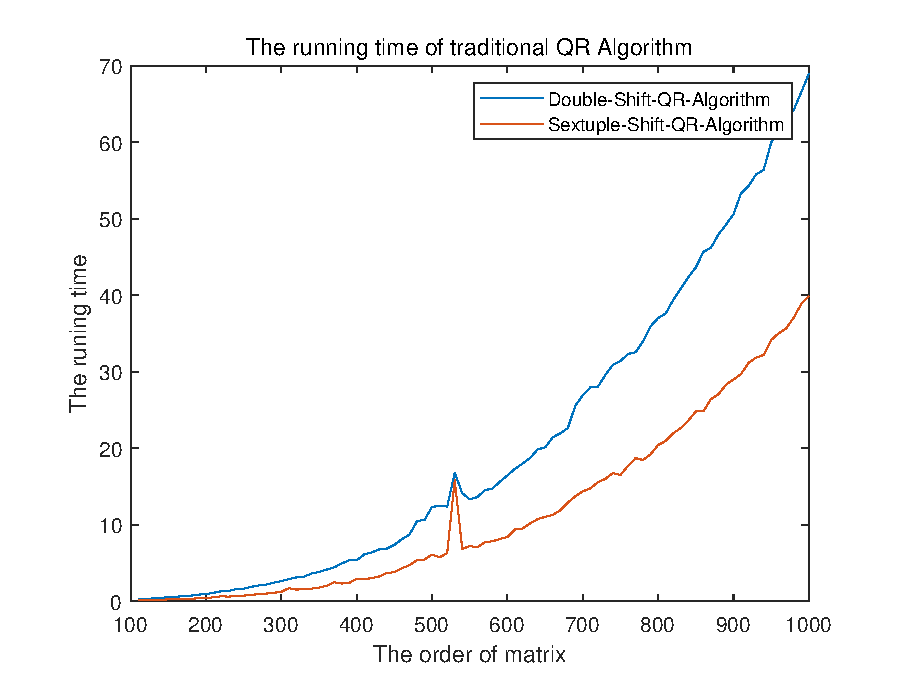
\includegraphics{The running time of traditional QR Algorithm.eps}
\caption{The running time of traditional QR Algorithm}
\label{1}
\end{figure}

This test can shows us that selecting more shifts every time can improve efficiency, so we propose multishift QR Algorithm, and choose small-bugle, which introduced two shifts each time. Then, add Aggressive Early Defaltion in and test again. This time it ranges from 620 to 1200 (since AED does not improve performance significantly in small matrices).
\begin{figure}[H]
\centering
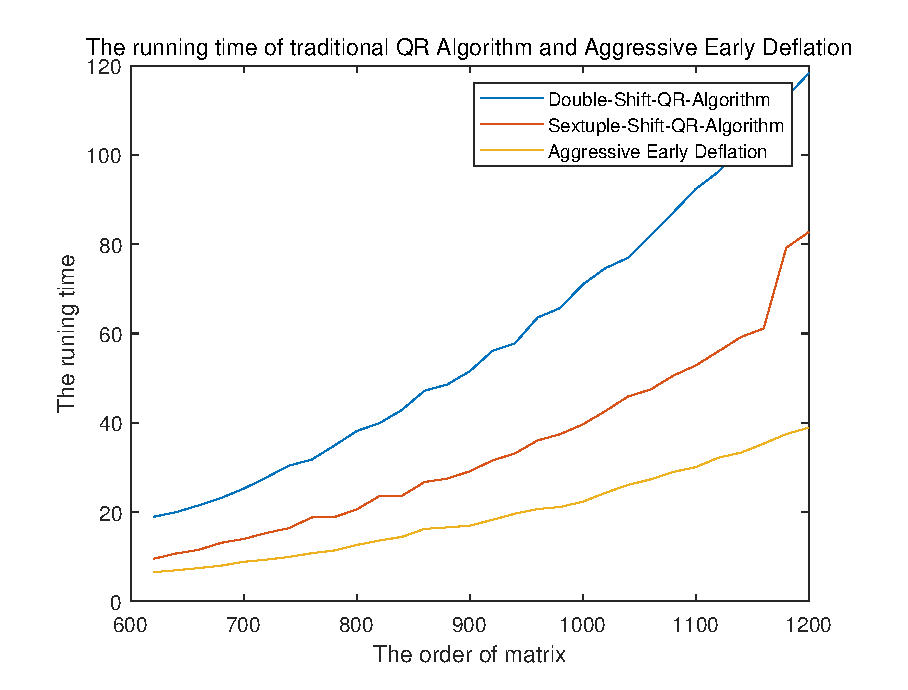
\includegraphics[height=10cm,width=15cm]{The running time of traditional QR Algorithm and Aggressive Early Deflation.eps}
\caption{The running time of traditional QR Algorithm and Aggressive Early Deflation}
\label{2}
\end{figure}

In the exploration function of Matlab, we can see that when the matrix order reaches 1000, the time required for hessenberg is close to that for AED processing. Now, we do a numerical experiment to prove it.
\begin{figure}[H]
\centering
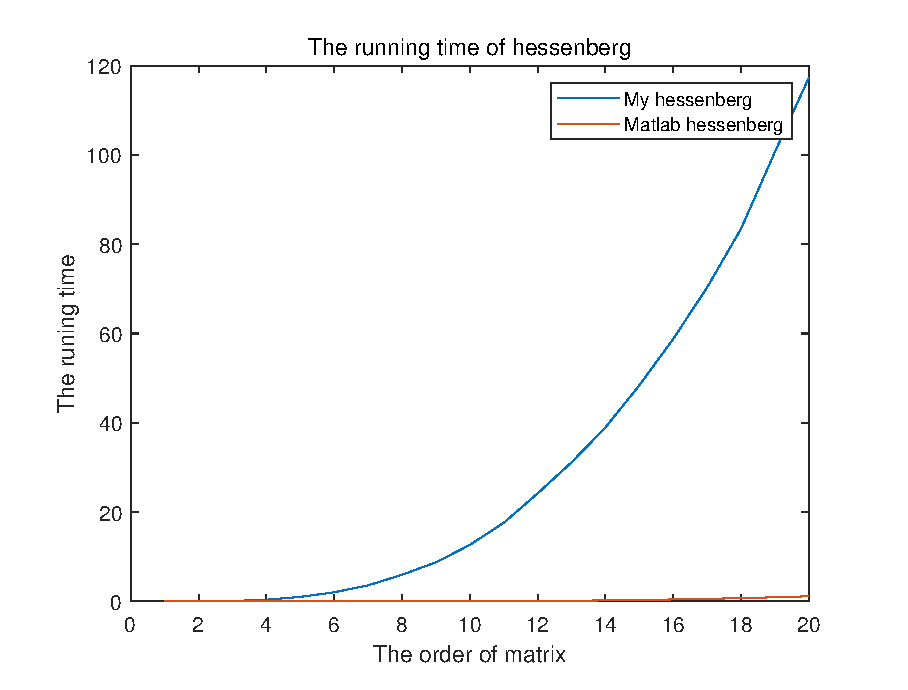
\includegraphics[height=10cm,width=15cm]{Hessenberg.eps}
\caption{The running time of Hessenberg and Matlab function}
\label{3}
\end{figure}

This can prove that the hessenberg program written by myself does not use BLAS-3 performance when dealing with thousands of matrices, so the performance will be much worse. Then, I use the built-in function \(hess\) to do following test.

Then we test Aggressive Early Defaltion with \(hess\) and the built-in function \(schur\), select a matrix from 1000 to 5350 and select one every 150.
\begin{figure}[H]
\centering
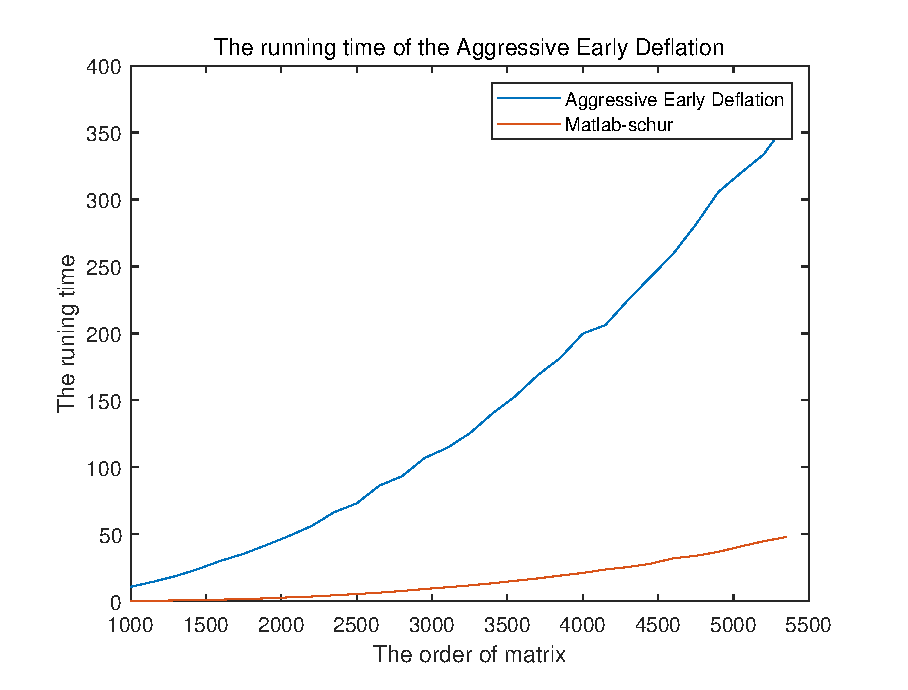
\includegraphics[height=10cm]{The running time of the Aggressive Early Deflation.eps}
\caption{The running time of the Aggressive Early Deflation}
\label{4}
\end{figure}

This test can shows us we can do a real-schur decomposition for a 5000*5000 matrix in about 6 minutes, then let us see the numerical stability.

We choose 23 matrices of order 500, change their condition number from \(10^3\) to \(10^14\) by singular value decomposition, then compute \(\frac{{{{\left\| {AQ - QH} \right\|}_F}}}{{{{\left\| A \right\|}_F}}}\) and \(\frac{{{{\left\| {{Q^T}Q - I} \right\|}_F}}}{{\sqrt n }}\) Then we can get:
\begin{figure}[H]
  \centering
  \subfigure[The numerical stability for schur decomposition]{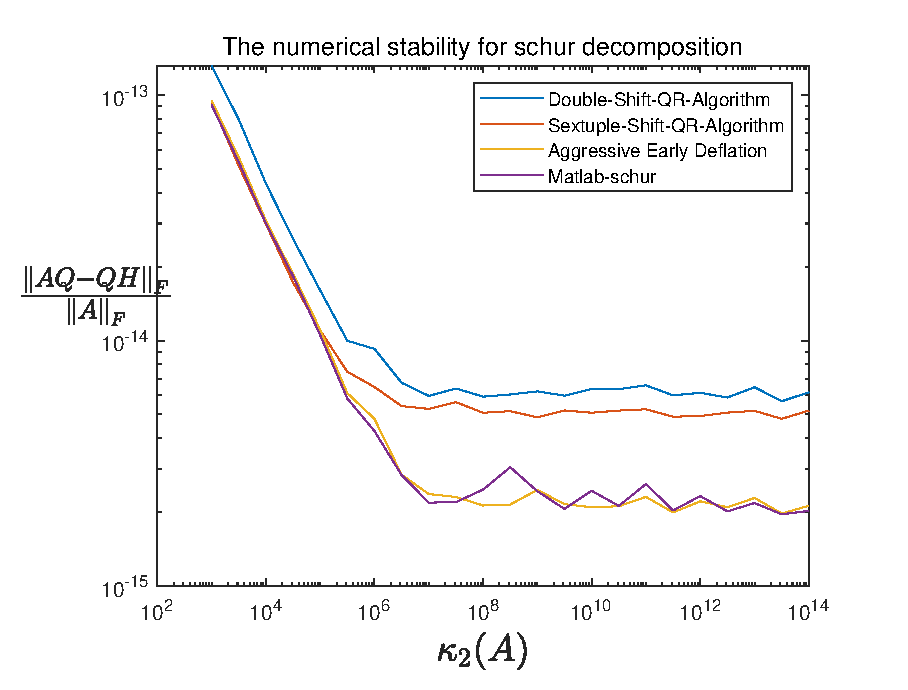
\includegraphics[width=3in]{The numerical stability for schur decomposition.eps}}
  \subfigure[The numerical stability for orthogonal matrix]{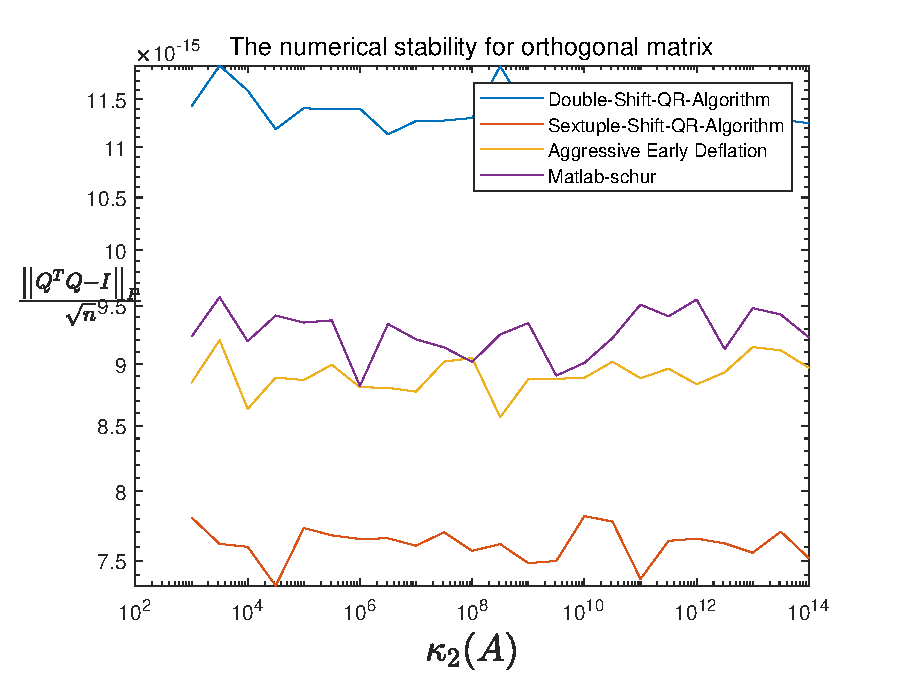
\includegraphics[width=3in]{The numerical stability for orthogonal matrix.eps}}
  \caption{The numerical stability}
\end{figure}

This can show us that the numerical stability is enough. I think maybe because of every orthogonal transformation is made with a home transformation.

As a reference standard, the information about the computer and the time to run the schur decomposition of the built-in matlab function will be given in the \textbf{The Appendix A} and all the matlab source code will be given in the \textbf{The Appendix B}.
\begin{appendix}
    \renewcommand{\thechapter}{\Alph{chapter}.}
    \chapter{Reference For Test}
    We test \(schur( )\) in Matlab as a reference, see the chart:
    \begin{table}[H]
\large
\begin{tabular}{|c|c|c|c|}
\hline
The order of matrix & The running time & The order of matrix & The running time \\ \hline
500                 & 0.6778           & 3500                & 14.6267          \\ \hline
1000                & 1.0522           & 4000                & 21.4383          \\ \hline
1500                & 1.1638           & 4500                & 29.2893          \\ \hline
2000                & 3.1954           & 5000                & 39.6178          \\ \hline
2500                & 6.4821           & 5500                & 53.0618          \\ \hline
3000                & 10.0568          & 6000                & 69.6150          \\ \hline
\end{tabular}
\end{table}
And the following chart shows the configuration of my computer
\begin{table}[H]
\large
\begin{tabular}{|c|c|}
\hline
CPU model       & Intel(R) Core(TM) i7-10750H CPU @ 2.60GHz \\ \hline
base frequency  & 2.6GHz                                    \\ \hline
turbo frequency & 5GHz                                      \\ \hline
Core number     & 6                                         \\ \hline
Threads number  & 12                                        \\ \hline
L1 cache        & 384kB                                     \\ \hline
L2 cache        & 1.5MB                                     \\ \hline
L3 cache        & 12.0MB                                    \\ \hline
Memory          & 32GB                                      \\ \hline
\end{tabular}
\end{table}
    \chapter{The Matlab Source Code}
    \lstinputlisting{household.m}
    \lstinputlisting{hessenberg.m}
    \lstinputlisting{double_shift_QR_iteration.m}
    \lstinputlisting{double_shift_QR_algorithm.m}
    \lstinputlisting{sextuple_shift_QR_iteration.m}
    \lstinputlisting{sextuple_shift_QR_algorithm.m}
    \lstinputlisting{double_shift_chasing_iteration.m}
    \lstinputlisting{eig_search.m}
    \lstinputlisting{choose.m}
    \lstinputlisting{aggressive_early_deflation.m}
    \lstinputlisting{project_traditional_running_time.m}
    \lstinputlisting{project_AED_running_time1.m}
    \lstinputlisting{project_hessenberg.m}
    \lstinputlisting{project_AED_running_time2.m}
    \lstinputlisting{project_the_numerical_stability.m}
\end{appendix}
\bibliography{reference}
\bibliographystyle{plain}
\end{document}
